\documentclass[tikz,border=10pt]{standalone}
\usepackage{helvet}
\renewcommand{\familydefault}{\sfdefault}
\usepackage{tikz}
\usetikzlibrary{arrows.meta, positioning, fit, calc, shapes.geometric, decorations.pathreplacing}

\definecolor{emeraldpine}{HTML}{1A4D3E}
\definecolor{harvardcrimson}{HTML}{A51C30}
\definecolor{ethdarkblue}{HTML}{1F407A}
\definecolor{ethpetrol}{HTML}{007A87}
\definecolor{ethbronze}{HTML}{B87333}
\definecolor{ethpurple}{HTML}{5B4B8A}
\definecolor{ink}{HTML}{1A202C}
\definecolor{softink}{HTML}{4A5568}
\definecolor{paleink}{HTML}{A0AEC0}
\definecolor{cardbg}{HTML}{F8FAFC}
\definecolor{shadecolor}{HTML}{F4F6F9}
\definecolor{ethpetrolbg}{HTML}{E3F3F5}
\definecolor{emeraldpinebg}{HTML}{E8F0EC}
\definecolor{ethbronzebg}{HTML}{F7EDE3}
\definecolor{linecolor}{HTML}{334155}

\begin{document}
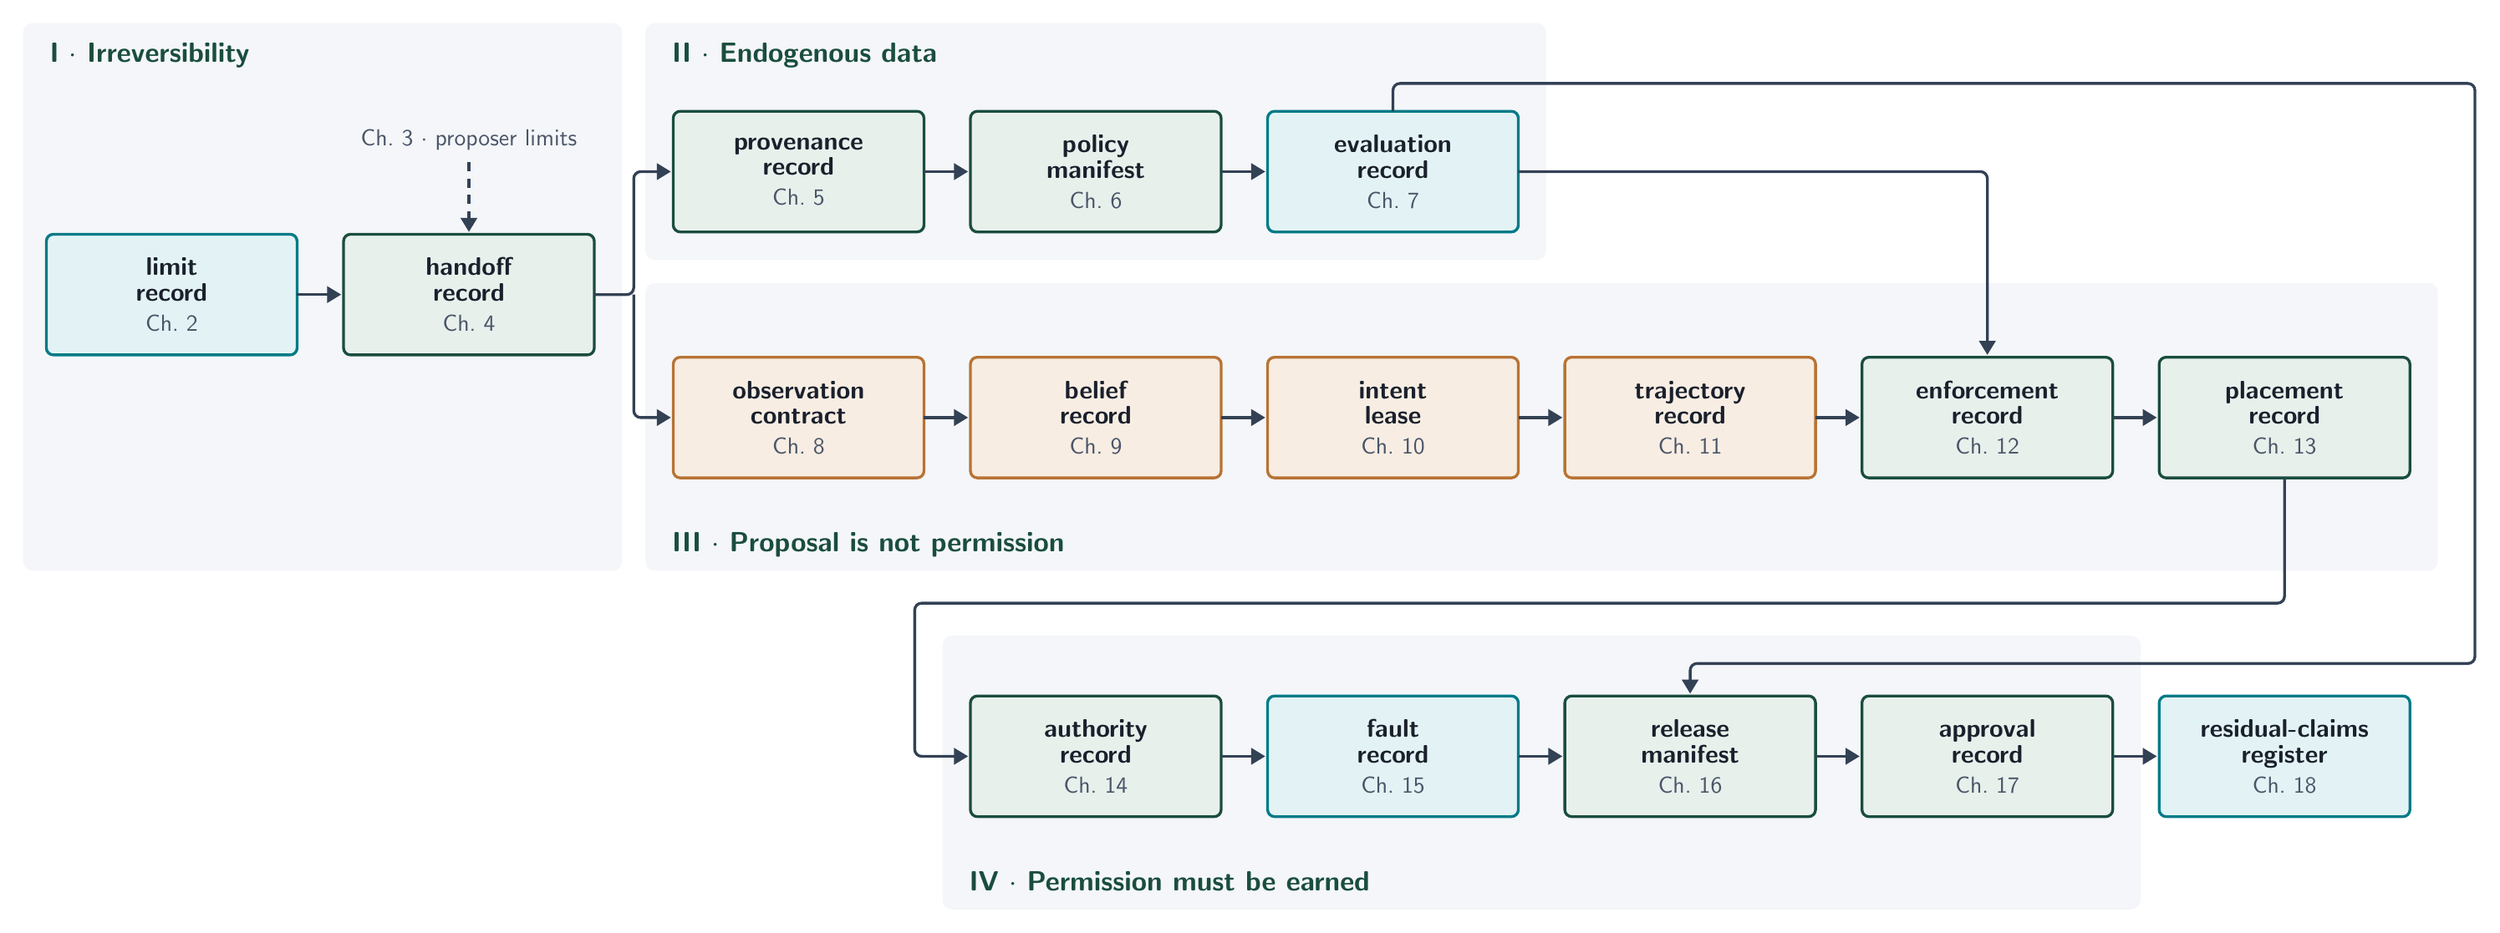
\begin{tikzpicture}[
    x=1bp, y=-1bp,
    >=Triangle,
    every node/.style={font=\sffamily},
    partband/.style={fill=shadecolor, rounded corners=4bp},
    box/.style={rounded corners=3bp, line width=1.2bp, align=center, inner sep=0},
    petrolbox/.style={box, fill=ethpetrolbg, draw=ethpetrol},
    pinebox/.style={box, fill=emeraldpinebg, draw=emeraldpine},
    bronzebox/.style={box, fill=ethbronzebg, draw=ethbronze},
    title/.style={font=\fontsize{11.5}{14}\bfseries, text=emeraldpine, anchor=base west},
    boxtext/.style={font=\fontsize{11}{13}\bfseries, text=ink},
    chaptext/.style={font=\fontsize{10}{12}\selectfont, text=softink},
    arr/.style={->, line width=1.2bp, draw=linecolor}
]

% Part bands (generated on one grid: boxes 108x52, column pitch 128)
\fill[partband] (30, 40) rectangle +(258, 236);
\fill[partband] (298, 40) rectangle +(388, 102);
\fill[partband] (298, 152) rectangle +(772, 124);
\fill[partband] (426, 304) rectangle +(516, 118);

\node[title] at (38, 57) {I $\cdot$ Irreversibility};
\node[title] at (306, 57) {II $\cdot$ Endogenous data};
\node[title] at (306, 268) {III $\cdot$ Proposal is not permission};
\node[title] at (434, 414) {IV $\cdot$ Permission must be earned};

\draw[petrolbox] (40, 131) rectangle +(108, 52) node[pos=.5, align=center] {
    \textcolor{ink}{\fontsize{11}{13}\bfseries limit}\\[-1bp]
    \textcolor{ink}{\fontsize{11}{13}\bfseries record}\\[1bp]
    \textcolor{softink}{\fontsize{10}{12}\selectfont Ch.\ 2}
};
\draw[pinebox] (168, 131) rectangle +(108, 52) node[pos=.5, align=center] {
    \textcolor{ink}{\fontsize{11}{13}\bfseries handoff}\\[-1bp]
    \textcolor{ink}{\fontsize{11}{13}\bfseries record}\\[1bp]
    \textcolor{softink}{\fontsize{10}{12}\selectfont Ch.\ 4}
};
\draw[pinebox] (310, 78) rectangle +(108, 52) node[pos=.5, align=center] {
    \textcolor{ink}{\fontsize{11}{13}\bfseries provenance}\\[-1bp]
    \textcolor{ink}{\fontsize{11}{13}\bfseries record}\\[1bp]
    \textcolor{softink}{\fontsize{10}{12}\selectfont Ch.\ 5}
};
\draw[pinebox] (438, 78) rectangle +(108, 52) node[pos=.5, align=center] {
    \textcolor{ink}{\fontsize{11}{13}\bfseries policy}\\[-1bp]
    \textcolor{ink}{\fontsize{11}{13}\bfseries manifest}\\[1bp]
    \textcolor{softink}{\fontsize{10}{12}\selectfont Ch.\ 6}
};
\draw[petrolbox] (566, 78) rectangle +(108, 52) node[pos=.5, align=center] {
    \textcolor{ink}{\fontsize{11}{13}\bfseries evaluation}\\[-1bp]
    \textcolor{ink}{\fontsize{11}{13}\bfseries record}\\[1bp]
    \textcolor{softink}{\fontsize{10}{12}\selectfont Ch.\ 7}
};
\draw[bronzebox] (310, 184) rectangle +(108, 52) node[pos=.5, align=center] {
    \textcolor{ink}{\fontsize{11}{13}\bfseries observation}\\[-1bp]
    \textcolor{ink}{\fontsize{11}{13}\bfseries contract}\\[1bp]
    \textcolor{softink}{\fontsize{10}{12}\selectfont Ch.\ 8}
};
\draw[bronzebox] (438, 184) rectangle +(108, 52) node[pos=.5, align=center] {
    \textcolor{ink}{\fontsize{11}{13}\bfseries belief}\\[-1bp]
    \textcolor{ink}{\fontsize{11}{13}\bfseries record}\\[1bp]
    \textcolor{softink}{\fontsize{10}{12}\selectfont Ch.\ 9}
};
\draw[bronzebox] (566, 184) rectangle +(108, 52) node[pos=.5, align=center] {
    \textcolor{ink}{\fontsize{11}{13}\bfseries intent}\\[-1bp]
    \textcolor{ink}{\fontsize{11}{13}\bfseries lease}\\[1bp]
    \textcolor{softink}{\fontsize{10}{12}\selectfont Ch.\ 10}
};
\draw[bronzebox] (694, 184) rectangle +(108, 52) node[pos=.5, align=center] {
    \textcolor{ink}{\fontsize{11}{13}\bfseries trajectory}\\[-1bp]
    \textcolor{ink}{\fontsize{11}{13}\bfseries record}\\[1bp]
    \textcolor{softink}{\fontsize{10}{12}\selectfont Ch.\ 11}
};
\draw[pinebox] (822, 184) rectangle +(108, 52) node[pos=.5, align=center] {
    \textcolor{ink}{\fontsize{11}{13}\bfseries enforcement}\\[-1bp]
    \textcolor{ink}{\fontsize{11}{13}\bfseries record}\\[1bp]
    \textcolor{softink}{\fontsize{10}{12}\selectfont Ch.\ 12}
};
\draw[pinebox] (950, 184) rectangle +(108, 52) node[pos=.5, align=center] {
    \textcolor{ink}{\fontsize{11}{13}\bfseries placement}\\[-1bp]
    \textcolor{ink}{\fontsize{11}{13}\bfseries record}\\[1bp]
    \textcolor{softink}{\fontsize{10}{12}\selectfont Ch.\ 13}
};
\draw[pinebox] (438, 330) rectangle +(108, 52) node[pos=.5, align=center] {
    \textcolor{ink}{\fontsize{11}{13}\bfseries authority}\\[-1bp]
    \textcolor{ink}{\fontsize{11}{13}\bfseries record}\\[1bp]
    \textcolor{softink}{\fontsize{10}{12}\selectfont Ch.\ 14}
};
\draw[petrolbox] (566, 330) rectangle +(108, 52) node[pos=.5, align=center] {
    \textcolor{ink}{\fontsize{11}{13}\bfseries fault}\\[-1bp]
    \textcolor{ink}{\fontsize{11}{13}\bfseries record}\\[1bp]
    \textcolor{softink}{\fontsize{10}{12}\selectfont Ch.\ 15}
};
\draw[pinebox] (694, 330) rectangle +(108, 52) node[pos=.5, align=center] {
    \textcolor{ink}{\fontsize{11}{13}\bfseries release}\\[-1bp]
    \textcolor{ink}{\fontsize{11}{13}\bfseries manifest}\\[1bp]
    \textcolor{softink}{\fontsize{10}{12}\selectfont Ch.\ 16}
};
\draw[pinebox] (822, 330) rectangle +(108, 52) node[pos=.5, align=center] {
    \textcolor{ink}{\fontsize{11}{13}\bfseries approval}\\[-1bp]
    \textcolor{ink}{\fontsize{11}{13}\bfseries record}\\[1bp]
    \textcolor{softink}{\fontsize{10}{12}\selectfont Ch.\ 17}
};
\draw[petrolbox] (950, 330) rectangle +(108, 52) node[pos=.5, align=center] {
    \textcolor{ink}{\fontsize{11}{13}\bfseries residual-claims}\\[-1bp]
    \textcolor{ink}{\fontsize{11}{13}\bfseries register}\\[1bp]
    \textcolor{softink}{\fontsize{10}{12}\selectfont Ch.\ 18}
};

\node[chaptext, anchor=base] at (222, 93) {Ch.\ 3 $\cdot$ proposer limits};
\draw[arr, dashed, dash pattern=on 4bp off 3bp] (222, 100) -- (222, 130);

% Arrows
\draw[arr] (148, 157) -- (167, 157);
\draw[arr, rounded corners=3bp] (276, 157) -- (293, 157) -- (293, 104) -- (309, 104);
\draw[arr, rounded corners=3bp] (293, 157) -- (293, 210) -- (309, 210);
\draw[arr] (418, 104) -- (437, 104);
\draw[arr] (546, 104) -- (565, 104);
\draw[arr] (418, 210) -- (437, 210);
\draw[arr] (546, 210) -- (565, 210);
\draw[arr] (674, 210) -- (693, 210);
\draw[arr] (802, 210) -- (821, 210);
\draw[arr] (930, 210) -- (949, 210);
\draw[arr] (546, 356) -- (565, 356);
\draw[arr] (674, 356) -- (693, 356);
\draw[arr] (802, 356) -- (821, 356);
\draw[arr] (930, 356) -- (949, 356);
\draw[arr, rounded corners=3bp] (674, 104) -- (876, 104) -- (876, 183);
\draw[arr, rounded corners=3bp] (1004, 236) -- (1004, 290) -- (414, 290) -- (414, 356) -- (437, 356);
\draw[arr, rounded corners=3bp] (620, 78) -- (620, 66) -- (1086, 66) -- (1086, 316) -- (748, 316) -- (748, 329);

\end{tikzpicture}
\end{document}
